\documentclass[tikz]{standalone}

% \usepackage{newtxtext,newtxmath}

%!TEX root = main.tex

% mytikzset
\usepackage{tikz}
\usetikzlibrary{positioning,arrows,shapes,patterns}
\usetikzlibrary{decorations.pathmorphing}
\usetikzlibrary{decorations.markings}
\usetikzlibrary{decorations.pathreplacing}
\usetikzlibrary{calc}
\usetikzlibrary{patterns}
\usetikzlibrary{decorations.markings}
\usetikzlibrary{petri}

\tikzset{
  vector/.style={thick,double,draw=black, postaction={decorate},
    decoration={markings,mark=at position .6 with {\arrow[black,scale=0.4]{triangle 45}}}},
  axial/.style={thick,double,densely dashed,draw=black, postaction={decorate},
    decoration={markings,mark=at position .6 with {\arrow[black,scale=0.4]{triangle 45}}}},
  gluon/.style={decorate, draw=black,
    decoration={coil,aspect=0.3,segment length=5pt,amplitude=3pt}},
  pseudo/.style={thick, dashed, draw=black, postaction={decorate},
    decoration={markings,mark=at position .6 with {\arrow[red,scale=0.5]{triangle 45}}}},
  scalar/.style={thick,draw=black, postaction={decorate},
    decoration={markings,mark=at position .6 with {\arrow[black,scale=0.5]{triangle 45}}}},
  cut/.style={draw=black, decorate, decoration={snake, segment length=1mm, amplitude=0.2mm}}
}

\usetikzlibrary{decorations.pathreplacing}

\begin{document}
\nopagecolor
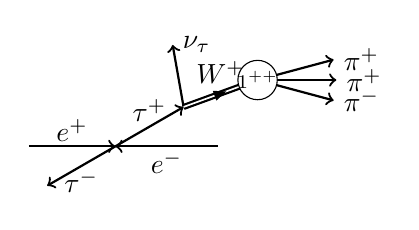
\begin{tikzpicture}[x=1cm,y=1cm]
      \draw[thick, ->] (-1.2+0.1,0) -- node[label={above,yshift=-2mm}:{$e^+$}] {} (0,0);
      \draw[thick, ->] ( 1.2+0.1,0) -- node[label={below,yshift=2mm}:{$e^-$}] {} (0,0);
      \draw[thick, ->] (0,0) -- node[label={above,yshift=-2mm}:{$\tau^+$}] {} ++(30:1);
      \draw[thick, ->] (0,0) -- node[label={below,yshift=2mm}:{$\tau^-$}] {} ++({180+30}:1);
      \draw[thick, ->] (30:1) -- ++(100:0.8) node[right] {$\nu_\tau$};
      \draw[vector   ] (30:1) -- node[coordinate, label=above:{$W^+$}] {} ++(20:1) node[] (a1) {};
      \draw[thick, ->] (a1) -- ++( 15:1) node[right] {$\pi^+$};
      \draw[thick, ->] (a1) -- ++(-15:1) node[right] {$\pi^-$};
      \draw[thick, ->] (a1) -- ++(  0:1) node[right] {$\pi^+$};
      \draw[draw, fill=white] (a1) circle (2.5mm) node[] {\scriptsize$1^{++}$};
\end{tikzpicture}
\end{document}
